\documentclass[letterpaper]{article}
\usepackage{proceed2e}
\usepackage[margin=1in]{geometry}
\usepackage{times}

\usepackage[utf8]{inputenc}
\usepackage[T1]{fontenc}

\usepackage{tikz}
\usetikzlibrary{calc}
\newcommand{\tikzmark}[1]{\tikz[overlay,remember picture] \node (#1) {};}
\newcommand{\underarrow}[2] {
  \begin{tikzpicture}[overlay,remember picture,out=340,in=210,distance=0.3cm]
    \draw [->,shorten >=3pt,shorten <=-3pt] ({#1}.south) to ({#2}.west);
  \end{tikzpicture}
  \hspace{-0.4cm}
}  
\newcommand{\Ex}{\mathbb{E}}
\usepackage{graphicx}
\usepackage{dblfloatfix}
%\usepackage[superscript,biblabel]{cite}
\usepackage{multirow,tabularx}
\usepackage{hhline}
\usepackage{amsmath}
\usepackage{cancel}

\usepackage[style=nature,
  citestyle=authoryear,
  maxcitenames=3,
  backend=biber,
  date=year]{biblatex}
%\bibliographystyle{apa}
\addbibresource{uiai.bib}

\newcommand\indep{\protect\mathpalette{\protect\independenT}{\perp}}
\def\independenT#1#2{\mathrel{\rlap{$#1#2$}\mkern2mu{#1#2}}}

\title{Inferring Causality from Finite Data using Conditional Independence}
%\author{Daniel Speyer\\Columbia University}
\author{}
\begin{document}

\maketitle

\begin{abstract}
  We propose techniques for inferring causal structure from limited
  observational data.  These techniques produce less extensive results
  than those which require exact joint probabilities, but are more
  practical.  The general principle is to describe multiple
  possible causal models in sufficient detail to have with specific
  consequences and test those
  consequences.  After developing these techniques abstractly, we test
  them in simulation and on real world Crohn's Disease data.
\end{abstract}

\section{Introduction}
Inferring causal graphs from observational data is a widely-sought
goal in statistics.  It is especially important in medicine, where
finding the cause of a disease may provide a way to cure or prevent
it, but finding an effect of a disease is of little practical value.
Medicine is also a context in which observational data is plentiful and finding
correlations is easy, but running intervention studies is slow,
expensive, regulated, and potentially dangerous.

The most common tool for causal inference is conditional
independence.  The specifics of a causal graph determine which node
are independent conditioned on which others by the ``bayes ball''
rule, and therefore it should be possible to observe the independences
and work backward to the causal graph.

This has proved to be more difficult in practice.  In particular,
observing independence is not as simple as it sounds.  [\cite{Pearl}] suggests
we test joint conditional probability distributions for equality.
Leaving aside the curse of dimensionality, this assumes we have the
exact distributions.  If all we have is a finite random sample from
those distributions, we can construct posteriors, but we cannot perform
an equality test.  [\cite{Spirtes}] encourage us to assume that
``the statistical decisions required by the [causal inference]
algorithms are correct
for the population'', while admitting that this requirement ``is often not met in
practice''.  Others have described this as ``possessing an
independence oracle'' [\cite{Peters,pcalg}].  Many simply include a
``test if $a\indep b|s$'' step in their algorithms, assuming the
reader will already know how.

In practice, the usual solution [\cite{akelleh,pcalg}] is to treat independence as a null
hypothesis, try to reject it at some p threshold, and treat any
failure as establishing it.  Needless to say, this is incorrect.
[\cite{bayesnet}] punts the responsibility to the caller instead,
which, while not actually wrong, is unhelpful

Dealing with finite data means the possibility of dealing with too
little data.  The elegant solution is to give some numerical
expression of confidence which becomes ``I don't know'' when the data
gets too small.  This solution has another benefit: in the biomedical
context, it is routine to test thousands of equally plausible
hypotheses at once.  A flat accuracy of 99\% is unhelpful in the face
of this, but a calibrated bayes factor allows compensation.

Traditional inference algorithms such as [\cite{Pearl}] generally
construct the entire DAG by a series of logical deductions that depend
on each other.  Such approaches do not translate easily to
uncertainty.  If we took the posterior probability for each
successive test in a traditional algorithm and multiplied them to get
a posterior for the entire graph, the resulting posterior would likely
be too low for any use, and might not be the overall plurality.
Furthermore, the number of possible causal graphs is roughly
exponential in the number of variables, so finding probabilities for
all of them is intractable outside of toy problems (even
\textit{storing} those probabilities is beyond the reach of real-world
hardware for most interesting problems in medicine!).

It may be possible to usefully approximate entire-DAG inference, but
we will attempt a less ambitious solution: to infer, as accurately as
possible, the direction of a single arrow.  Specifically, one pointing
from a variable we can easily intervene on (a ``cure'') to one we care
about (a ``disease'').

\subsection{Motivating Problem: Crohn's Disease}

This paper is optimized around a specific practical problem:
untangling the microbiome's role in Illial Crohn's Disease.  It is
well established that there are many differences in the intestinal
bacteria of healthy people and of people with the disease
[\cite{hofer}], but it is not established which (if any) of the differences of
bacteria \textit{cause} the disease.  
There have been attempts to determine this by randomized controlled
trial, but early results are discouraging [\cite{rctma}] and the number
of species, combined with other relevant
variables, make exhaustive RCTs impractical.

Data is available on this problem from [\cite{data}], including
genetic, microbiome and
health information, but for only 58 patients (plus another 24 with
microbiome and health information, but not genetic).  The microbiome
information is a series of 16S reads, but can generally be described
as ``present'' or ``absent'', with very low concentrations of a
species rounded off to ``absent''.  This comes much closer to fitting
the empirical distributions than any simple scalar formula, which is
why this paper uses binary variables.

\section{Collider Finding}

Let us begin with the simplest case.  Suppose we have a known cause, a
known effect, and a variable which connects to the effect in an
unknown way.   For Crohn's Disease, the known cause is mutations in the NOD2
gene [\cite{nod2}], the known effect is the disease, and the unknown
is each of 222 species of plausibly relevant bacteria, taken
independently.  To help keep our example in mind, we will refer to
these factors as $G$ (``gene''), $D$ (``disease'') and $B$
(``bacterium'').  So our initial graph is $G \rightarrow D$ -- $B$.
We do not observe a
correlation between $G$ and $B$, but that might only mean our test is
underpowered.  

For now, we will assume that there is no direct causal
link between $G$ and $B$, and furthermore that there are no unobserved
confounders or selection effects.  We will consider these later.
This leaves us only two models, $G \rightarrow D \rightarrow B$ or $G
\rightarrow D \leftarrow B$.  We can call these ``chain'' and
``collide'' models, or $m_{ch}$ and $m_{co}$ for short.  Can we
distinguish between them?

Yes.  Let us consider
$p(G,B)$:

\begin{eqnarray*}
p(G,B|m_{ch}) & = & \sum_D p(G)p(D|G)p(B|D) \\
p(G,B|m_{co}) & = & p(G)p(B)
\end{eqnarray*}

We do not actually know the terms on the right side of those
equations, so let us parameterize both models with $\theta$ and
rewrite the equations as:


\begin{multline*}
  p(G,B|m_{ch}) = \\
  \int \left ( \sum_D p(G|\theta) p(D|G,\theta) 
  p(B|D,\theta) \right ) p(\theta) d\theta \\
  p(G,B|m_{co}) = \int p(G|\theta)p(B|\theta)p(\theta) d\theta
\end{multline*}

We can learn $p(\theta)$ from available data using dirichlet priors.
The integrals would be difficult algebraically, but they can be
adequately approximated with monte-carlo sampling.

Once we have these, let $n_{g,b}$ be the count of datapoints with
G=g,B=b and we can use:

\begin{equation*}
p(n_*|m) \propto \prod_{g,b} p(g,b|m)^{n_{g,b}}
\end{equation*}

This is proportional instead of equal because there is a combinatoric term,
but it cancels when taking odds ratios so it can be safely ignored.
From here, we can apply standard bayesian updating.

\subsection{Without a Known Cause}

Suppose we do not have a link of known direction.  If we can find two
variables $B_1$ and $B_2$ such that both correlate to $D$ but not to
each other, then the only simple causal graph that could generate this
is $B_1 \rightarrow D \leftarrow B_2$.  This finds two causes.

Just as we looked at $p(G,B)$ in the previous case, here we look at
$p(B_1,B_2)$.  The competing hypothesis $B_1 \rightarrow D \rightarrow
B_2$ is the same as before, but we must now consider $B_1 \leftarrow D
\rightarrow B_2$ (let us call this the ``V'' model).  In fact, we can
use the exact same formula:

\begin{eqnarray*}
  p(B_1,B_2|m_v)
  & = & \sum_D p(B_1|D)p(B_2|D)p(D) \\
  & = & \sum_D \frac{p(B_1,D)}{p(D)}\frac{p(B_2,D)}{p(D)}p(D) \\
  & = & \sum_D \frac{p(B_1,D)p(B_2,D)}{p(D)} \\
  & = & \sum_D \frac{p(B_1)}{p(B_1)}\frac{p(D,B_1)}{1}\frac{p(B_2,D)}{p(D)} \\
  & = & \sum_D p(B_1)p(D|B_1)p(B_2|D) \\
  & = & p(B_1,B_2|m_{ch})
\end{eqnarray*}

There is also the possiblity of $B_1\rightarrow B_2 \rightarrow D$,
but in this case the $B_1-B_2$ link will be stronger than the $B_1-D$
link, so there is no risk of a false collider.

There is also the possibility of non-simple-connectedness.  For
boolean $D$, if there are many variable $B_{1..n}$ that strongly
influence it, they \textit{must} correlate to each other.  Otherwise
they would be responsible for more than all of the variation in $D$.
Fortunately, the common case here will result in false negatives.

\subsection{Non-Simply-Connected Graphs}

What if there is a causal effect $G\rightarrow B$?  It must be weak
enough not to be detected, but that doesn't say much.  Let us consider
it by cases.

\subsubsection{False Colliders}

Can a true graph of
$G\tikzmark{a}\rightarrow D \rightarrow{B}\tikzmark{c}$
\underarrow{a}{c}
produce a $p(G,B)$ more similar to a graph
$G \rightarrow D \leftarrow B$?  This would require the direct and
indirect influence of $G$ on $B$ to cancel out rather precisely.  If
the indirect influence is stronger, we will pick the correct model,
albeit underconfidently.  If the direct influence is too strong, we
will see a correlation between $G$ and $B$.  And if the direct
influence is in the same direction as the indirect, the correct model
will remain the better fit (though both models will be worse).

\subsubsection{False Chains}

Similarly, can a true graph of
$G\tikzmark{a2}\rightarrow D \leftarrow{B}\tikzmark{c2}$
\underarrow{a2}{c2}
produce a $p(G,B)$ more similar to a graph
$G \rightarrow D \rightarrow B$?  Again, this is possible, but there
is no reason for $p(B|G)$ to resemble $\sum_D p(B|D)p(D|G)$.  If
$p(B|G)-p(B|\bar{G})$ is too large, $G\not\indep B$ will be detected
initially, whereas if it's too small, the correct model will be
chosen.  Furthermore, what shrinks the upper bound is for the
predicted $G-B$ relation in the chain model to be small, which also
means any erroneous bayes factor will be small.

\subsection{Unobserved Confounders}

This technique is vulnerable to confounders.  Specifically, if the
$D-B$ link is the product of a common cause, that will generate no
$G-B$ dependence, exactly like a collider.  That is, it will suggest
we ought to use that bacterium as a treatment, though in fact doing so
would be ineffective.

This risk is increased by using a two-bacterium approach, as
\textit{either} link being the result of a confounder invalidates our
conclusions about both links.

\section{D-Separation}

Ideally, we'd like to answer questions of the form
$A\overset{?}{\indep}B|S$, not just find individual colliders.
It is probably
impossible for a formula to say that $A\not\indep B$ in full
generality, but it may be possible to say $A\not\indep B|S$
sufficiently for our purposes.

Suppose $A$, $B$ and $S$ are variables already known to correlate.  The simplest
associated models are $S-A-B$, $A-S-B$ and $A-B-S$, where $S$ severs only in
the $A-S-B$ case (the directions on the arrows are not important at the
moment, except that there can be no colliders).  For the first two
models:

\begin{eqnarray*}
  p(A,B|S,m_{\cancel{sever}}) & = & p(A|S)p(B|A) \\
  p(A,B|S,m_{sever}) & = & p(A|S)p(B|S)
\end{eqnarray*}

And there is a symmetric formula for the last one.  Since there are
two alternative hypotheses, we take whichever produces the greater
probability.  Somewhat surprisingly, there is no advantage here in
using monte-carlo posteriors instead of simple maximum likelihood estimators
for the conditional probabilities.

There is another simple causal graph that can cause three variables to
correlate: all could be influenced by a common confounder $H$ (for
``hidden'').  This case is impossible to test for in full generality,
because $S$ could follow $H$ so closely as to be an acceptable proxy,
and therefore controlling for $S$ effectively controls for $H$.  In
theory, it should be possible to infer $H$ and its conditionals usings
a Gibbs-sampler-like system.  In practice, there is more room to
overfit this more complex model and no straightforward way to
compensate.  What does work surprisingly well is to ignore this case
and apply the exact same test as before.

\subsection{Applying D-Separation}

If we are willing to trust the d-separation test, can we use it to find
causes of a variable of interest?  Deducing the entire causal graph
is a brittle endevour, but there is a local solution.

Suppose there exist three variable (bacteria) with a common (hidden) cause,
such that one causes the variable of interest (disease), that is
$H \rightarrow \tikzmark{h} B_1 \rightarrow D \; B_2\tikzmark{b3} \;
B_3\tikzmark{c3}$ \underarrow{h}{b3} \underarrow{h}{c3}.  The trio
$B_{1,2,3}$ can be identified because they
all correlate and remain correlated when controlling for any of them.
No special test is needed for this, standard $\chi^2$ can produce a p
value for all of this.  The role of $B_1$ can be identified because it
severs $B_2$ and $B_3$ from $D$.  No other simply connected graph has
these properties.

Note that this does not attempt to find \textit{all} causes of $D$,
only those for which suitable $H$, $B_2$ and $B_3$ exist.

\subsubsection{Application to Genomic Studies}

The causal graph mentioned above is a common one in genome-wide
association studies, where the hidden factor is population structure,
the three correlating variables are genetic features and the variable
of interest is a phenotype.  The goal, once again, is to determine
\textit{which} generic feature directly affects the phenotype.  One
answer is that it is the one which best separates the others from the
phenotype, and that this can be measured with the same formulas as
here.

Whether this will produce useful results in practice is a question for
a later study.

\subsection{Unobserved Confounders}

This technique is robust against unobserved confounders.  If the links
between $H$ and $B_{1-3}$ in the preceding graph are
actually mutual effect from a confounder, then that confounder can be
thought of as a part of $H$ (which is itself unobserved).  If the link
between $B_1$ and $D$ is via confounder, then there will be no
$B_{2,3}-D$ correlations to seperate.

\subsection{Non-Simply-Connected Graphs}

These techniques depend on simply-connected graphs.  Both the d-separation
test and its application can say nothing of significance in the face
of multiple connections.

\section{Parsimony}

Given that it will be necessary to assume either ``no unobserved
confounders'' or ``simple connection'', can we at least say that these
are the most parsimonious explanations for our data?

From a graphical model perspective, they are not.  It is the absence
of a link which is a statement about the world.

From a biochemical perspective, they are.  Each link asserts an
interaction, and the default for organic molecules or micro-organisms
is not to interact with each other.  As for unobserved confounders, the
presence of unobserved variables in biology is a given, but for them
to be confounders requires \textit{two} interactions that relate to
each other.

Fields other than biology will need to reconsider this.

\section{Testing in Simulation}

\begin{figure}[b!]
  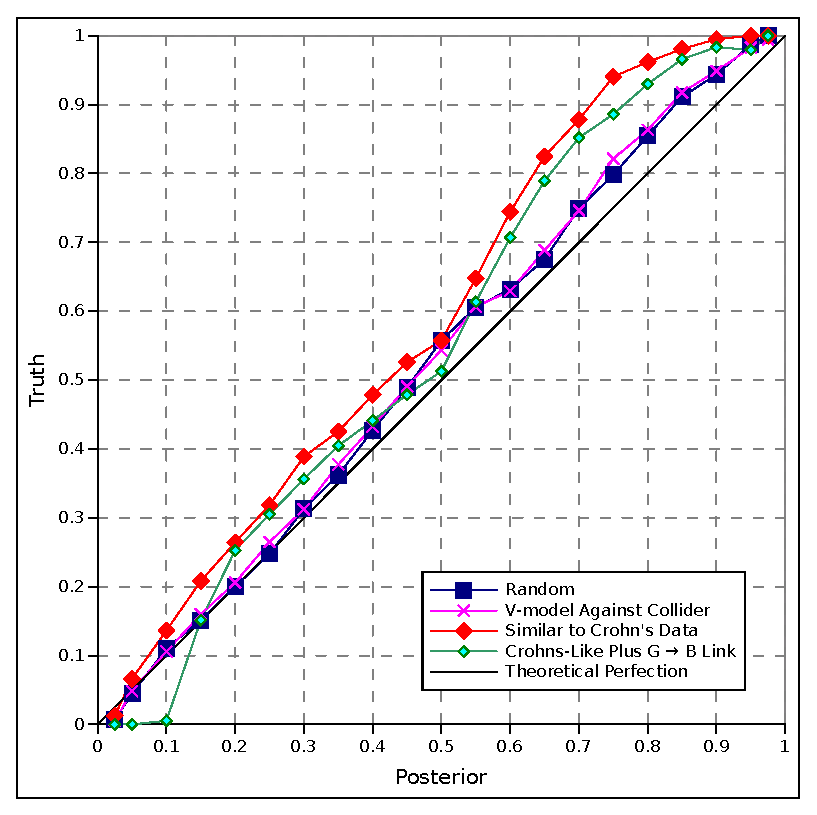
\includegraphics[width=.5\textwidth]{test_direction_uni}
  \caption{Simulated data using 100k chain and collide models, each
    generating 58 datapoints.
    Higher numbers indicate collider.  Blue squares indicate
    parameters drawn from a flat distribution.  Purple Xs indicate the
    same, except discerning colliders from v models instead of
    chains. Red diamonds indicate a
    Crohn's-like distribution ($p(G)$ and $p(D|G)$ taken from
    data; $G\indep B$ and $D\not\indep B$ `shown' by $\chi^2$ test,
    $p>0.1$ and $p<0.01$ respectively).  Open green diamonds indicate
    the same, except with a $G\rightarrow B$ link in the true causal
    model (still $p>0.1$).}
  
  \label{dir_pla58}
\end{figure}

\begin{figure}
  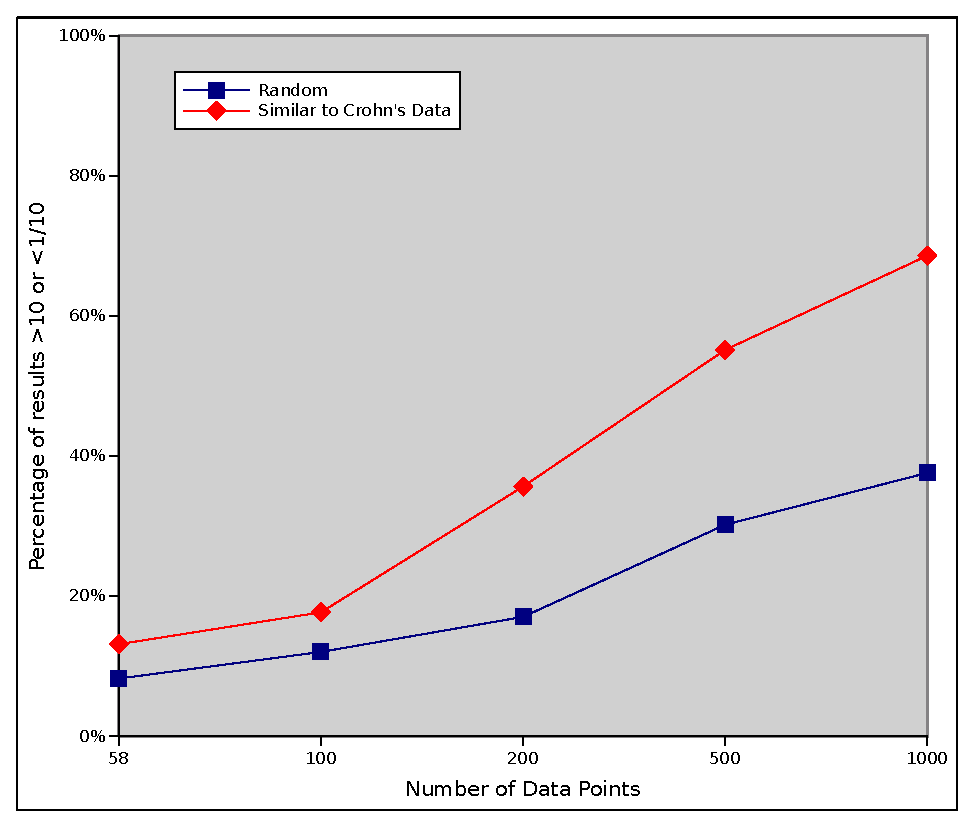
\includegraphics[width=.5\textwidth]{usefullness}
  \caption{Fraction of bayes factors that were at least 10:1 one way
    or the other as a function of dataset size, for the
    collider-detection test.}
  \label{dir_use}
\end{figure}

\begin{figure}
  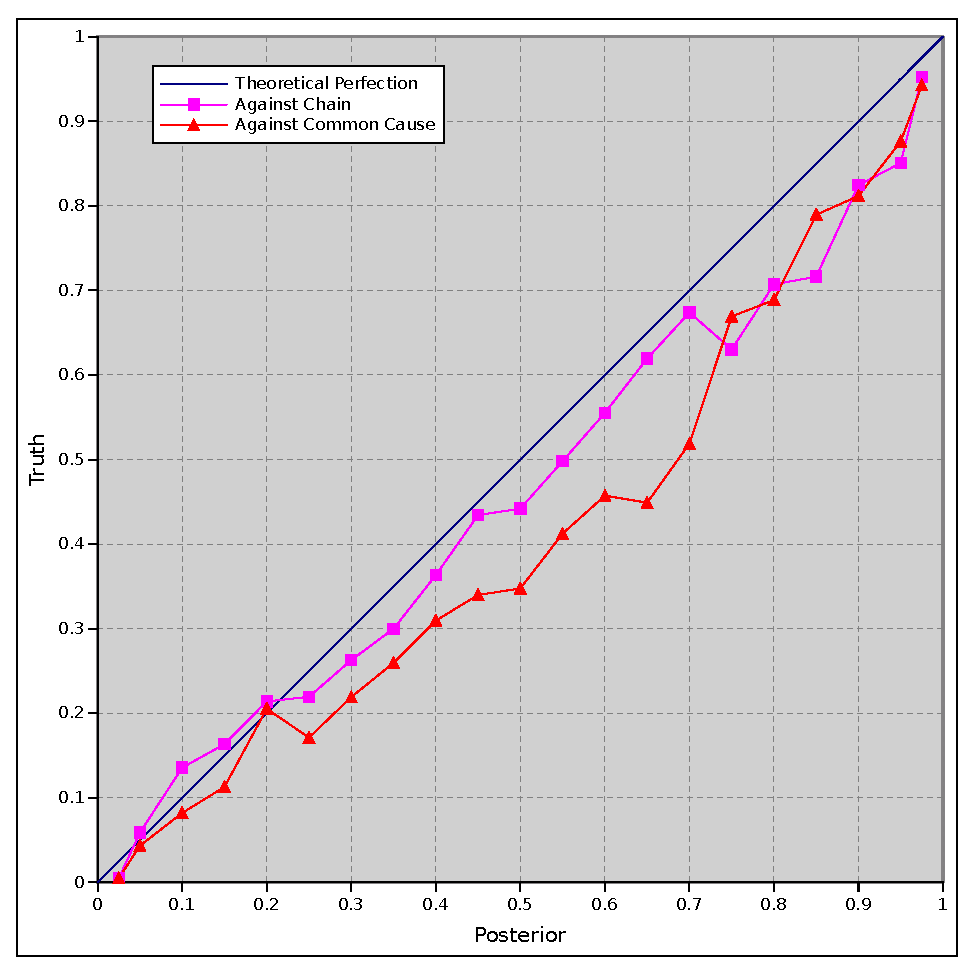
\includegraphics[width=.5\textwidth]{sever}
  \caption{Calibration for the d-separation test, both in the case it was
    designed for and in the case of comparing severing to common
    cause.  Higher probabilities indicate separation.}
  \label{sever}
\end{figure}

\begin{figure*}
  \begin{tabular}{llrr}
    Species & Sick When & P-Value ICD link & Bayes Factor Causality \\
    Streptococcus pseudopneumoniae & $>$6.36E-05 & 3.1e-05 & 5.15 \\
    Streptococcus infantis & present & 0.0014 & 2.55 \\
    Lactobacillus acidophilus & $>$8.15E-05 & 0.00017 & 10.64 \\
    Sphingopyxis alaskensis & present & 0.0004 & 2.43 \\
    Clostridium methylpentosum & $\leq$6.31E-04 & 0.00085 & 2.53 \\
    Roseiflexus castenholzii & present & 7.3e-05 & 3.30 \\
    Ruminococcus faecis & $\leq$1.07E-03 & 0.0022 & 2.40 \\
  \end{tabular}
  \caption{Results of the direction test on 222 interesting species,
    using $\chi^2$ to check a relationship to Crohn's Disease and the
    direction test described here to establish that it causes (or
    prevents) the disease.}
  \label{dir_tab}
\end{figure*}

\begin{figure*}[b]
  \begin{tabular}{llllllr}
Species 1 & Sick When & p.v. & Species 2 & Sick When & p.v. & B.F \\
    Lawsonia intracellularis & $\leq1.3\mathrm{e}{-4}$ & $0.004$ & Sporobacter termitidis & $\leq2.5\mathrm{e}{-4}$ & $4\mathrm{e}{-6}$ & 4.5 \\
Anoxybacillus thermarum & present & $1\mathrm{e}{-6}$ & Ruminococcus albus & $\leq1.2\mathrm{e}{-4}$ & $0.004$ & 4.5 \\
Hespellia stercorisuis & $\leq9.9\mathrm{e}{-5}$ & $0.002$ & Ralstonia solanacearum & $\leq1.7\mathrm{e}{-2}$ & $0.004$ & 4.4 \\
Clostridium xylanolyticum & $\leq1.2\mathrm{e}{-3}$ & $0.001$ & Ralstonia solanacearum & $\leq1.7\mathrm{e}{-2}$ & $0.004$ & 4.2 \\
Anoxybacillus flavithermus & $>1.7\mathrm{e}{-4}$ & $1\mathrm{e}{-6}$ & Eubacterium siraeum & $\leq9.9\mathrm{e}{-5}$ & $0.0002$ & 4.1 \\
Anoxybacillus thermarum & present & $1\mathrm{e}{-6}$ & Coprococcus eutactus & $\leq1.6\mathrm{e}{-4}$ & $0.0002$ & 5.9 \\
Anoxybacillus flavithermus & $>1.7\mathrm{e}{-4}$ & $1\mathrm{e}{-6}$ & Coprococcus eutactus & $\leq1.6\mathrm{e}{-4}$ & $0.0002$ & 5.3 \\
Anoxybacillus kamchatkensis & present & $3\mathrm{e}{-5}$ & Gemmiger formicilis & $\leq8.7\mathrm{e}{-4}$ & $5\mathrm{e}{-6}$ & 8.5 \\
  \end{tabular}
  \caption{Results of collider-search looking for pairs of bacteria.
    The ``sick when''  column indicates when that species is
    associated with disease and the ``p.v.'' column the p-value
    showing that association ($\chi^2$ test).  The ``B.F.'' column
    gives the bayes factor for the collider model as opposed to chain
    or v.}
  \label{two_bact_tab}
\end{figure*}

\begin{figure*}
  \begin{tabular}{llllr}
    Species & Sick When & Severs & Third in Trio & Bayes Factor \\
    Coprococcus catus & $\leq$2.67E-04 & B intestinihominis & O splanchnicus & 33.34 \\
Faecalibacterium prausnitzii & $\leq$1.43E-02 & B xylanolyticus & P hordei & 28.48 \\
Flavobacterium thermophilum & $>$2.23E-04 & S infantis & A flavithermus & 83.28 \\
Clostridium glycyrrhizinilyticum & $\leq$4.84E-04 & R faecis & A johnsonii & 46.54 \\
Eubacterium oxidoreducens & $\leq$1.57E-03 & C eutactus & C cellobioparum & 32.67 \\
Bacteroides helcogenes & $\leq$5.10E-04 & L crispatus & B helcogenes & 18.03 \\
Anoxybacillus flavithermus & $>$2.97E-04 & G subterraneus & F thermophilum & 337.11 \\
Clostridium formicaceticum & $\leq$1.74E-04 & A indistinctus & F prausnitzii & 13.29 \\
Streptococcus oralis & $>$1.07E-04 & S sanguinis & V dispar & 13.49 \\
Sporobacter termitidis & $\leq$2.47E-04 & E ruminantium & T forsythia & 106.95 \\
  \end{tabular}
  \caption{Incomplete output of the trio-and-sever test.  All trios
    established p<0.01.  The first species is the one that appears to
    impact Crohn's Disease; the second is the one that the correlates
    with disease until the first is controlled for, and the third is a
    third with a common cause.}
  \label{sev_tab}
\end{figure*}

To test these tools, we created causal networks with the structures we
sought to distinguish, filling in the parameters at random.  Then we
used each net to create a dataset, and used the dataset to infer the
shape of the net.  We used the fraction of nets of each shape as a
prior and used that to convert the bayes factor into a posterior,
which we compared to the true shape of the net.

We calculated the mean log error, that is, we took the probability the
system assigned to the correct shape, took its negative natural log,
and took the mean of those over all generated nets.  Always being
certain and correct would be an error of 0, whereas ever being certain
and wrong would be an error of infinity.

We also drew calibration graphs.  For these, we gathered test nets by
their posteriors (in buckets 5 percentage points wide) and calculated
the actual percentage of each shape for nets in a bucket.  A perfectly
calibrated test is one such that of all the nets it assigns a 85\%
probability of being colliders, 85\% of them actually are.

\subsection{Collider Detection}

This test is well-calibrated over random parameters, as shown by
figure \ref{dir_pla58}, but with only 58 datapoints, the vast majority
of nets return bayes factors close to 1.  Only 8\% of nets produce
bayes factors outside the [0.1, 10] range.  The average log error is
0.62, roughly the same as if it had returned a posterior of 0.5 for
everything.

This is not terribly surprising.  58 datapoints is not very much
data.  Any statistical test would be hard-pressed to report useful
conclusions from that except in the presence of strong trends, which
randomly-drawn parameters rarely produce.  That the test correctly
identifies what it does not know is good, but not very useful.

Increasing the size of the dataset helps (see figure \ref{dir_use}).
At 1000 datapoints, 38\% of results are outside that range, and the
average log error drops to 0.42. Obtaining 1000s patients'
microbiome data might be expensive (though dropping rapidly, as
direct-to-consumer microbiome sequencing becomes available), but
obtaining similar epidemiological data is common.

We also tested this using data more similar to the Crohn's Disease
dataset.  We generated nets using real-world $p(G)$ and $p(D|G)$ with
random bacterial parameters.  Then we filtered them to only include
nets where $B \not\indep D$ was detectable by $\chi^2$ test $p<0.01$,
and to not include any where $G \not\indep B$ was detectable by
$\chi^2$ test $p<0.1$.  The 
former is a test we would apply anyway (it is not useful to determine
causality of a link that may not exist!) and the latter is a cheap
test that does not rule out a significant number of species.  The
calibration is slightly worse as judged by the graph, though average
log loss is lower 0.59 at 58 datapoints, 0.23 at 1000, and the
tendency to produce useful results increases by almost a factor of 2.
This is because the Crohn's-like generation rules out several
scenarios about which nothing useful can be said, such a too-weak
$B-D$ link, or a $p(G)$ so high or low that the other case cannot be
analyzed.

Finally, we tested the system using nets that have a $G\rightarrow B$
link, albeit one that cannot be detected by $\chi^2$ test
($p\not<0.1$).  As expected, this produced a moderate general trend to
underconfidence, but still a mostly well-calibrated result.

In every case, the error at the high end was in the direction of
underconfidence.  As the high end corresponds to clinical
applicability, this means that we will occasionally miss an effective
therapy that an ideal algorithm would have found, but we will not
claim an ineffective therapy is effective (any more than normal
uncertainty requires).

\subsection{D-Separation}

The d-separation test has mean log loss of 0.41 when comparing a
separator to a chain (that is, $A-S-B$ vs $A-B-S$) and 0.49 when
comparing to a common, hidden cause ($A-S-B$ vs $H-A,B,S$).  Both
follow close to a straight line (see figure \ref{sever}).

The applied severing technique does not try to find \textit{all}
causes of $D$, only
those which happen to fit this motif and are strong enough for a
$\chi^2$ test to pick up.  As such, it is unclear what it would mean
to test it in simulation.  Certainly with parameters chosen for the
purpose, it will work.  With random parameters, it will generally fail
to find trios.

\subsection{Common Cause Testing}

The test for three variables with a common cause is simple: test each
pair for dependence using standard $\chi^2$ both with and without
controlling for the third.  If all six tests find a p-value under the
threshold, consider them common-caused.

This test does not attempt to find all trios with common causes.  For
random parameters, it will find very few.  To test it, we created
exceptionally strong links, by drawing $p(B|A)$ from either [0,0.25]
or [0.75,1] and $p(B|~A)$ from the other range.  With these links, and
a p-threshold of 0.001, we found the following results:

  \begin{tabular}{lrrr}
    Number of datapoints & 58 & 100 & 500 \\
    $H \tikzmark{h5} \rightarrow A \; B\tikzmark{b5} \; C\tikzmark{c5}$
    \underarrow{h5}{b5} \underarrow{h5}{c5} &
    16.6\% & 56\% & 99.4\% \\
    $ A \rightarrow B \rightarrow C $ &
    8.8\% & 9.6\% & 2.9\%
  \end{tabular}

This shows the Common Cause Test works, at least for strong links, but
only with larger datasets than we actually have.




\section{Crohn's Disease}

Returning to the original motivating problem, what do these techniques
show for Crohn's Disease?

First we converted the lists of reads into boolean
values.  We converted each read to a species names using BLAST [\cite{BLAST}]
and the 16S Microbial database [\cite{16S}].  For each read, we
selected the highest-matching species (an imperfect, but unbiased
technique) and dropped all reads without matches.  We divided by total
reads to get a concentration.  For each species, we chose a threshold that
maximized the number of Crohn's Disease statuses that could be
correctly predicted by that bacterium alone.  Finally, we compared the
concentrations to the thresholds to produce boolean values. These
boolean values can then be thought of as ``has a clinically relevant
dosage of the bacterium''.

Once the values were booleanized, all those with
entropies less than 0.5 were dropped on the logic that a species
that's always the same can't have a clinical effect.  This left 222
species, of which 61 showed correlation to Crohn's Disease $(p<0.01)$
and did not show correlation to NOD2 $(p\cancel{<}0.1)$.

Of these the collider-finding test against the NOD2 gene found 8 which
show signs of impacting
Crohn's Disease, though only one (Lactobacillus acidophilus) has a
bayes factor greater than 10.  The 8 are shown in figure \ref{dir_tab}.

Inconveniently, that species appears to
be \textit{harmful}, which is surprising given the usual role of
lactobacilli but less so given that two RCTs found this same result
(albeit nonsignificantly) [\cite{lgg1,lgg2}].  It may be relevant that
L. acidophilus is usually found in the
\textit{jejunum} [\cite{lacid}], but these samples are from
\textit{ileum} biopsies.  Perhaps the cause of Crohn's Disease is not
which bacteria are in the intestine, but where in the intestine they
are.  This result is inconvenient because removing or moving bacteria
is far more difficult than adding them.

Could this be the result of a direct $G\rightarrow B$ link?  In this
case, the generally
understood role of NOD2 as mediating \textit{untargetted} immune
responses [\cite{nod2}], makes that unlikely.

Looking for two-bacterium colliders, we find 8 pairs with bayes
factors above 4, containing 13 species (3 of them twice).  This is
shown in figure \ref{two_bact_tab}.  To a degree, the number of pairs
we did \textit{not} find is disturbing, but the number of strongly
causal species means there \textit{must} be hidden common causes.

The d-separation three-species test offers more possible species (see figure
\ref{sev_tab}).  The bayes factors are higher, but the overall
complexity of the test is reason to be nervous.  This test also took
extremely long to run, which may require fixing before it can be used
seriously.

The species without strong bayes factors are still encouraging.  The
p-value confirms they relate to Crohn's Disease in some way, in which
case ``causes'' and ``is caused by'' are the most likely models by
simple priors.  These small values bump our posterior belief some.
This is not enough to recommend to patients, but it is a better place
to start RCTs than anything we had before.

\subsection{Adjusting for Multiple Hypotheses}

\begin{figure}[b!]
  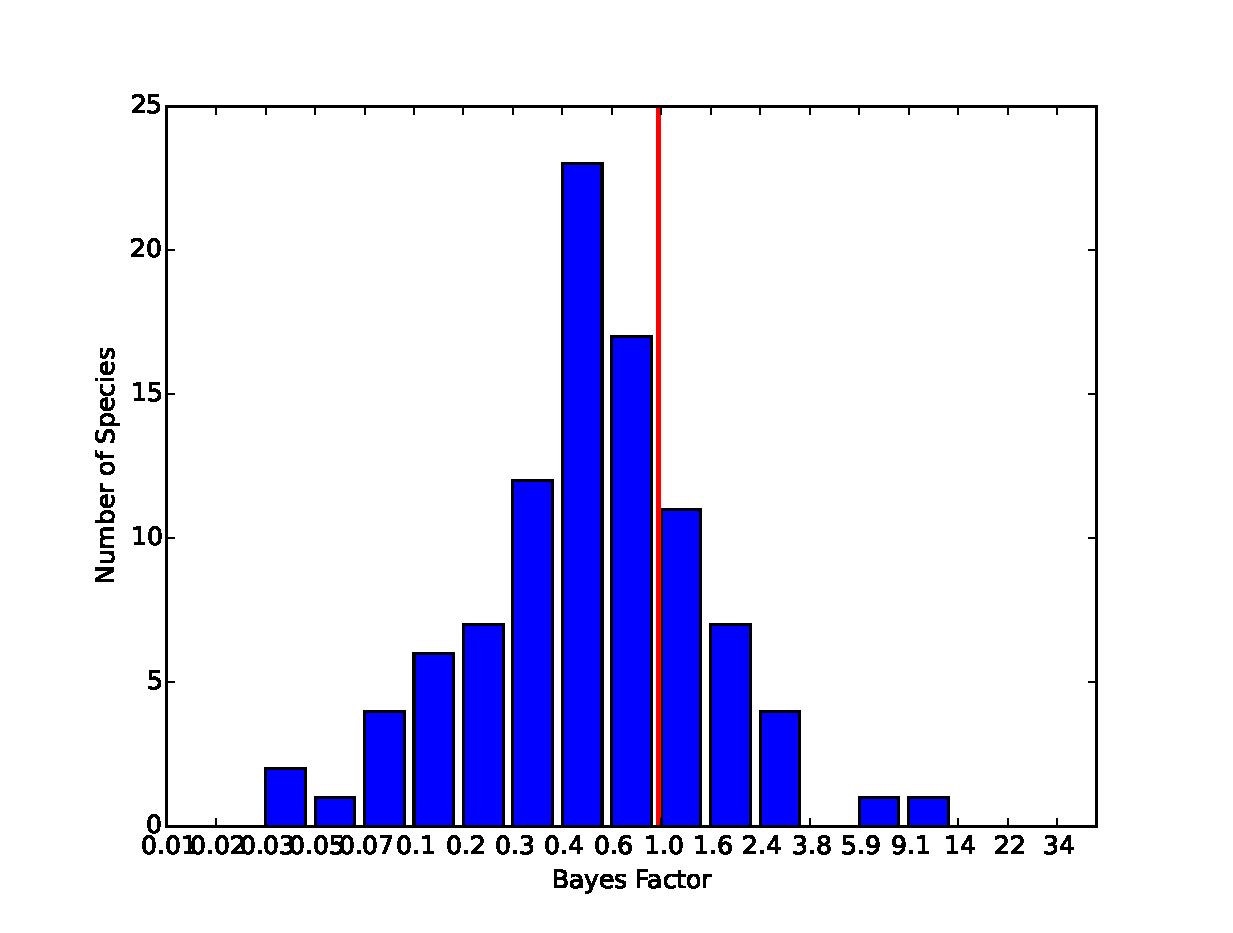
\includegraphics[width=0.5\textwidth]{histogram}
  \caption{Number of correlating species with each bayes factor
    (higher means cause, lower means effect) as found by the gene
    collision test.}
  \label{hist}
\end{figure}

Having considered 61 species of bacteria in order to find any that
appear causal must cast some doubt on our results.  Worse, considering
1830 pairs of species for the Bacterium-Bacterium Collider or almost
36 thousand triples for the Applied D-Separation test case extreme
doubt.

The classic response to this problem would be to divide our prior by
the number of hypotheses, similarly to a Bonferroni correction.  This
would represent our a-priori knowledge that exactly one of the species
under consideration is causal.  In fact, we know nothing of the sort.
Different species of bacteria routinely emit similar chemical signals,
and likely play similar biological roles.

What do we know a-priori?  For any given correlating species, a 50\%
prior credence of causality sounds reasonable, albeit debatable.  A
99.9\% confidence that between 20 and 50 of the species are causal
most emphatically does not.  A different prior does not protect us
from this class of absurdity.  The only reasonable conclusion is that
our uncertainties regarding different species are not independent of
one another.  Specifically, each time we learn the causal nature of a
single correlating species, we should update our belief in the others
in the same direction.  This makes sense biologically, since some of
our uncertainty about different species stems from the same unknowns
in human biology.

Sadly, this does not give us a numeric answer, but it does encourage
us to look at the histogram (figure \ref{hist}).  We see a clear peak on the
``weak evidence for disease $\rightarrow$ bacteria'' side, and most of
the species over the line look like the spread around the peak.
L. acidophilus and S. pseudopneumoniae appear to be outliers, and
therefore more likely to be real causal effects.

The same technique cannot be applied to the Two Bacterium Collider
test, because any common cause of the species (that is, 
$H\tikzmark{h4} \rightarrow B_1,\tikzmark{b14} B_2\tikzmark{b24}
\rightarrow D\tikzmark{d4}$ \underarrow{h4}{b24} \underarrow{b14}{d4})
will produce a correlation between $B_1$ and $B_2$ despite their
collider nature.   Since $H$ can be literally \textit{any}
environmental factor that effects both species, its presence is less
of a possibility and more of an inevitability.
\printbibliography

\end{document}
